% LTeX: language=it

\subsection{Problema 1}
Possiamo inizialmente visualizzare la curva di nostro interesse in un piano cartesiano tridimensionale:
\begin{center}
    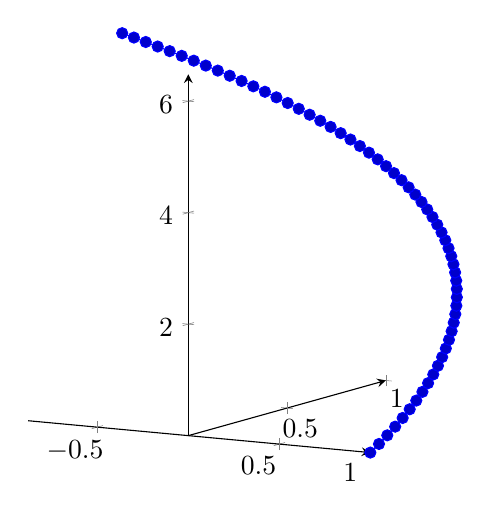
\begin{tikzpicture}
        \begin{axis}[
                view={30}{10},
                axis lines=center,
            ]
            \addplot3+[domain=0:sqrt(7),samples=60,samples y=0]
            ({cos(deg(x))},
            {sin(deg(x))},
            {sqrt(6)*x});
        \end{axis}
    \end{tikzpicture}

    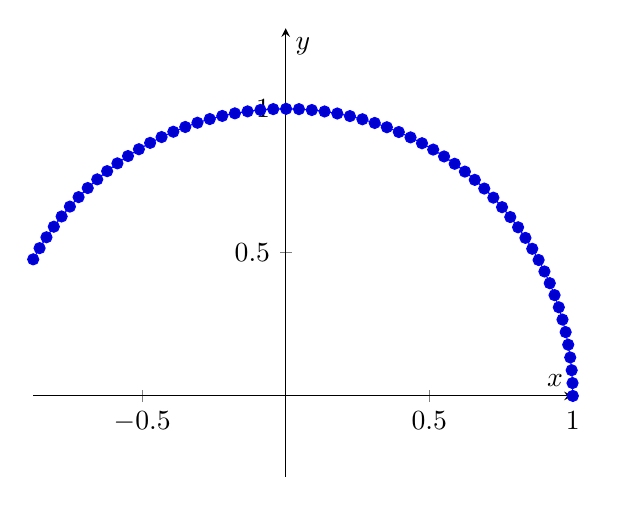
\begin{tikzpicture}
        \begin{axis}[
                view={0}{90},
                axis lines=center,
                xlabel=$x$,
                ylabel=$y$,
                zlabel=$z$,
                axis equal
            ]
            \addplot3+[domain=0:sqrt(7),samples=60,samples y=0]
            ({cos(deg(x))},
            {sin(deg(x))},
            {sqrt(6)*x});
        \end{axis}
    \end{tikzpicture}
\end{center}

\noindent Si procede ora al calcolo della lunghezza della curva come:
\begin{equation}
    \int_{0}^{\sqrt{7}} \sqrt{\left(\frac{dx}{dt}\right)^2 + \left(\frac{dy}{dt}\right)^2 + \left(\frac{dz}{dt}\right)^2} dt
\end{equation}
Si procede ora al calcolo delle derivate:
\begin{equation}
    \begin{split}
        \frac{dx}{dt} = -\sin(t) \\
        \frac{dy}{dt} = \cos(t)  \\
        \frac{dz}{dt} = \sqrt{6}
    \end{split}
\end{equation}
Si procede ora al calcolo della lunghezza della curva:
\begin{equation}
    \begin{split}
        \int_{0}^{\sqrt{7}} \sqrt{(-\sin(t))^2 + (\cos(t))^2 + (\sqrt{6})^2} dt = \\
        = \int_{0}^{\sqrt{7}} \sqrt{1 + 6} dt = \sqrt{7} \int_{0}^{\sqrt{7}} dt = \sqrt{7} \sqrt{7} = 7
    \end{split}
\end{equation}